\documentclass[11pt]{article}

\usepackage[margin=1in]{geometry}
\usepackage{amsmath, amssymb, amsthm}
\usepackage{graphicx}
\usepackage{booktabs}
\usepackage{enumitem}
\usepackage{hyperref}
\usepackage{setspace}
\usepackage{natbib}
\usepackage{xcolor}
\usepackage{caption}
\usepackage{subcaption}
\usepackage{multirow}
\usepackage{authblk}

\setstretch{1.1}

% NeurIPS-style paragraph spacing: no indent, small skip between paragraphs.
\setlength{\parindent}{0pt}
\setlength{\parskip}{0.6em}

% Theorem environments
\theoremstyle{plain}
\newtheorem{theorem}{Theorem}
\newtheorem{lemma}[theorem]{Lemma}
\newtheorem{proposition}[theorem]{Proposition}
\theoremstyle{definition}
\newtheorem{definition}[theorem]{Definition}

% Shorthand
\newcommand{\E}{\mathbb{E}}
\newcommand{\R}{\mathbb{R}}
\newcommand{\fjac}{J_{f_\theta}}
\newcommand{\NFE}{\mathrm{NFE}}

\hypersetup{
  colorlinks=true,
  linkcolor=blue!50!black,
  citecolor=blue!50!black,
  urlcolor=blue!50!black
}

\title{When Does Jacobian Regularization Engage in Neural ODEs? \\
  A Penalty--Fit--Stiffness Trade-off}
\author[1]{Athena Zhuoming Zhong}
\affil[1]{University of Pennsylvania, ENM 5220 Numerical Methods for PDEs}
\date{Apr 2026}

\begin{document}

\maketitle

\begin{abstract}
Jacobian regularization is a standard tool for taming the solver cost of Neural
Ordinary Differential Equations (Neural ODEs)~\citep{finlay2020train}, but its
behaviour on stiff target systems is not well-characterised. We run a 115-cell
empirical study on Van der Pol and harmonic oscillator targets, sweeping the
penalty weight $\lambda_J \in \{0, 10^{-3}, 10^{-2}, 10^{-1}\}$ where
applicable, the Hutchinson sample count $K \in \{1, 4\}$, the stiffness
parameter $\mu \in \{10, 25, 50, 100\}$, and the adaptive-solver tolerance
$r_\text{tol} \in \{10^{-3}, 10^{-5}, 10^{-7}\}$. Our central finding is an
\textbf{engagement gap}: at $\mu = 10$ (the better-fit setting, validation
$\mathrm{MSE} = 1.18$) the penalty
reduces the learned Jacobian Frobenius norm by $10.4\%$ at $\lambda_J = 10^{-1}$;
at $\mu = 50$ (the poorer-fit setting, $\mathrm{MSE} = 1.94$) the same
penalty produces only a $1.0\%$ change. The preregistered interaction
hypothesis H1 ($\Delta\NFE_\text{stiff} > \Delta\NFE_\text{smooth}$) is
therefore \emph{not} supported in these runs: the penalty engages in a
non-stiff, better-fit regime and is inert in a stiffer, poorer-fit regime. As
an ancillary comparison, an unregularised explicit adaptive solver is
wall-clock about $6.9\times$--$7.9\times$ faster than a fixed-point implicit
method at matched validation MSE on Van der Pol, with the apparent advantage
growing with $\mu$ (uncorrected one-sided Wilcoxon $p = 0.031$ at each
$\mu \in \{25, 50, 100\}$; none survives Bonferroni correction across the
three-comparison family). At $\mu = 100$ both solvers integrate a poorly-fit
network, so this is matched-bad MSE rather than matched-good MSE. Finally, the
observed NFE ratio is consistent with the order-$5$ Runge--Kutta accuracy bound
$\NFE \propto r_\text{tol}^{-1/6}$: tightening $r_\text{tol}$ by four decades
grows NFE by $5.54\times$, close to the predicted $4.64\times$, and the fitted
exponent is $0.186$ versus the theoretical $1/6$. We close with the
\emph{penalty--fit--stiffness trade-off} these findings suggest: Jacobian
regularization helps in the better-fit, non-stiff regime and fails to engage in
the poorer-fit, stiffer regime.
\end{abstract}

\section{Introduction}
\label{sec:intro}

Neural ODEs~\citep{chen2018neural} replace discrete residual updates with a
continuous-time dynamical system $\dot x = f_\theta(x, t)$, $x(0) = x_0$, and
compute the forward pass by numerically integrating $f_\theta$ from $t = 0$ to
$t = T$. This decoupling has consequences that classical numerical analysis
predicts: a model can be expressive enough to fit the task while still inducing
a vector field that is expensive to integrate, either because its Jacobian is
large (truncation error dominates) or because its spectral radius is large
(stability bounds the step size). \citet{finlay2020train} address the first
problem by adding a soft Frobenius-norm penalty on $\fjac$ to the training
loss; they report reductions in the number of solver function evaluations
(NFE) on density-estimation tasks. \citet{kim2021stiff} document the second
problem: stiff Neural ODEs are difficult to train at all, since fast and slow
modes drive the optimiser in conflicting directions.

\paragraph{Original question and pivot.}
This work began with a question at the intersection of those two literatures:
\emph{does the NFE benefit of Jacobian regularization depend on the stiffness
of the underlying dynamics?} The proposal preregistered three hypotheses: an
interaction hypothesis (\textbf{H1}) predicting larger NFE reductions on
stiff targets, a stiffness-suppression hypothesis (\textbf{H2}), and an
ancillary hypothesis (\textbf{H3}) comparing explicit-regularized against
implicit-unregularized integration. The preregistered $2{\times}2{\times}2$
factorial returned a null on H1 and H2; the diagnosis --- three follow-up
sweeps over $\lambda_J$, $K$, and $\mu$ --- became the paper. We find an
\emph{engagement gap}: at $\mu = 10$ the penalty engages cleanly, at $\mu = 50$
it is operationally inert, and the contrast appears tied to model fit quality.
We interpret this as a \emph{penalty--fit--stiffness trade-off} in this
experimental setup: regularization requires fit, while increasing target
stiffness coincides with poorer fit under standard training, so the engagement
regime and the stiffness regime do not overlap here
(\S\ref{sec:discussion}).

\paragraph{Contributions.}
\begin{enumerate}[leftmargin=2em]
\item \textbf{An engagement gap for Jacobian regularization} (\S\ref{sec:engagement}).
  We show that whether the Frobenius penalty shapes $f_\theta$ depends
  on whether the model has fit the target well enough to develop a high-norm
  Jacobian. At $\mu = 10$ the penalty engages cleanly; at $\mu = 50$ it does
  not, across the tested $\lambda_J \in \{0, 10^{-3}, 10^{-2}, 10^{-1}\}$
  settings and a $K=4$ Hutchinson check.
\item \textbf{A penalty--fit--stiffness trade-off that explains the null}
  (\S\ref{sec:null}, \S\ref{sec:discussion}). The originally-preregistered
  H1 and H2 are not supported; we give a back-of-envelope mechanism in terms
  of the penalty-to-task gradient ratio, and show that the engagement and
  stiffness regimes do not overlap on this task family.
\item \textbf{A tolerance-scaling ratio consistent with the order-$p$ accuracy bound}
  (\S\ref{sec:h0}). A four-decade tolerance tightening grows NFE by $5.54\times$
  (theory predicts $4.64\times$); the fitted exponent is $0.186$, close to the
  theoretical $1/6$, but the sweep co-scales $a_\text{tol}$ and retrains each
  tolerance cell, so we treat it as a consistency check rather than an isolated
  eval-time tolerance law.
\item \textbf{An implicit-vs-explicit comparison with a stiffness slope}
  (\S\ref{sec:h3}). On Van der Pol at matched validation MSE, an explicit
  adaptive solver is about $6.9\times$--$7.9\times$ faster wall-clock than the
  fixed-point implicit method in \texttt{torchdiffeq}, with the apparent
  advantage growing as $\mu$ increases --- although at $\mu = 100$ the
  matched-MSE precondition holds only because both solvers integrate a
  poorly-fit network.
\end{enumerate}

\section{Background and Related Work}
\label{sec:background}

\paragraph{Neural ODEs.}
The continuous-depth viewpoint of \citet{chen2018neural} treats a residual block
as an Euler step on a learned vector field. Training requires backpropagation
through an ODE solver, which is handled either via the adjoint method
(memory-efficient, but precludes certain regularizers) or by direct
backpropagation through the discretization (heavier memory cost, but
differentiable through any per-step computation).

\paragraph{Jacobian and kinetic regularization.}
\citet{finlay2020train} introduce two regularization terms motivated by
optimal-transport theory: a kinetic energy $\int_0^T \|f_\theta(x_t, t)\|^2 dt$
that encourages low-velocity flows, and a Jacobian Frobenius penalty
$\int_0^T \|\fjac(x_t, t)\|_F^2 dt$ that encourages low-Lipschitz flows. Their
key empirical claim is that simpler flows can be integrated with fewer solver
evaluations without sacrificing density-estimation
performance~\citep{grathwohl2019ffjord}. The penalty is computed in practice
via Hutchinson's stochastic trace estimator~\citep{hutchinson1990stochastic}:
$\E_\epsilon[\|\fjac^\top \epsilon\|^2] = \|\fjac\|_F^2$ when
$\E[\epsilon\epsilon^\top] = I$, which costs a single vector--Jacobian product
per sample.

\paragraph{Stiff Neural ODEs.}
\citet{kim2021stiff} study Neural ODE training when the target system has
widely separated time scales (e.g., Robertson kinetics~\citep{robertson1966solution}).
They report that gradient descent fails on stiff systems even with implicit
solvers, attributing the failure to gradient instability from the
adjoint-system stiffness. Our work confirms a complementary failure mode:
even when training does not diverge, the network may simply collapse to a
low-norm vector field that fails to reproduce the stiff dynamics, leaving the
Jacobian penalty with nothing to suppress.

\paragraph{Step-size theory.}
The classical Hairer--N\o{}rsett--Wanner treatment~\citep{hairer1993solving,
hairer1996solving} distinguishes two regimes for explicit Runge--Kutta cost.
In the accuracy-limited regime, an order-$p$ embedded method takes
$N \propto T \cdot M^{p/(p+1)} \cdot \tau^{-1/(p+1)}$ steps where $M$ bounds
the $(p{+}1)$-th derivative of the solution; in the stability-limited regime
on a stiff problem, $N \propto T \cdot \rho(J)/C_p$ where $\rho(J)$ is the
spectral radius of the Jacobian and $C_p$ is method-dependent. These bounds
underlie our predictions for both H0 (\S\ref{sec:h0}) and the conditional
interaction \eqref{eq:interaction-prediction} in Appendix~\ref{app:interaction}.

\paragraph{Implicit integration.}
The Dahlquist barrier~\citep{dahlquist1963special} establishes that
$A$-stability is incompatible with linear-multistep methods of order
$> 2$. Implicit Runge--Kutta methods such as Radau IIA and Kvaerno do
achieve $A$- and $L$-stability at higher order but require Newton iteration
per step. \citet{rackauckas2017differentialequations} provide a mature Julia
ecosystem for these solvers; our work uses the simpler fixed-point implicit
Adams in torchdiffeq~\citep{chen2018torchdiffeq} as the implicit baseline and
notes the limitations of this choice in \S\ref{sec:limitations}.

\section{Methods}
\label{sec:methods}

\subsection{Tasks and ground-truth trajectories}
\label{sec:tasks}

We use two ground-truth dynamical systems:

\paragraph{Harmonic oscillator (smooth control).}
The damped linear oscillator $\ddot x_1 + 2\gamma \dot x_1 + \omega^2 x_1 = 0$,
written as a first-order system with $x = (x_1, x_2)$, $\dot x_1 = x_2$,
$\dot x_2 = -\omega^2 x_1 - 2\gamma x_2$, with $\omega = 1$, $\gamma = 0.1$.
The Jacobian is constant; the analytic solution provides a known-correct
reference.

\paragraph{Van der Pol oscillator (parameterised stiffness).}
The classical relaxation oscillator~\citep{vanderpol1926relaxation}
$\dot x_1 = x_2$, $\dot x_2 = \mu (1 - x_1^2) x_2 - x_1$. The stiffness
ratio scales with $\mu$. We use $\mu \in \{10, 25, 50, 100\}$, where
$\mu = 50$ is the proposal's preregistered ``mildly stiff'' setting and
the other values are added post-hoc to characterise the engagement regime
and to test the H3 stiffness slope.

For each system, $n_\text{train} = 256$ and $n_\text{val} = 64$ initial
conditions are sampled as $x_0 \sim x_0^\star + 0.1 \cdot \mathcal{N}(0, I_2)$,
with $x_0^\star = (1, 0)$ (harmonic) or $(2, 0)$ (Van der Pol). Reference
trajectories are integrated with \texttt{torchdiffeq.odeint} using
\texttt{dopri5}, $r_\text{tol} = 10^{-9}$, $a_\text{tol} = 10^{-11}$, which is
four orders of magnitude tighter than any training-time solver tolerance.

\subsection{Neural ODE model}
\label{sec:model}

The vector field $f_\theta \colon \R \times \R^2 \to \R^2$ is a multilayer
perceptron with two hidden layers of width 64 and $\tanh$ activations
(4{,}610 parameters). Time is provided as an explicit feature: the network
input is $[x, t] \in \R^3$. The model is trained to regress trajectories: a
forward pass calls $\texttt{torchdiffeq.odeint}(f_\theta, x_0, t)$ to obtain
$(T, B, 2)$ predicted trajectories, and the loss is
$\mathcal{L}_\text{task} = (\hat x - x)^2$ averaged over time, batch, and
state dimensions.

\subsection{Jacobian regularization}
\label{sec:reg}

When $\lambda_J > 0$, the training loss is augmented with
\begin{equation}
\mathcal{L}_\text{total} = \mathcal{L}_\text{task}
  + \lambda_J \cdot \E_{(x, t) \sim \mu_\text{train}}
    \!\left[\|\fjac(x, t)\|_F^2\right],
\label{eq:loss}
\end{equation}
where $\mu_\text{train}$ is the empirical distribution over ground-truth
training trajectory points; 32 such points are sampled per training step. The
Frobenius norm is estimated by the Hutchinson
estimator~\citep{hutchinson1990stochastic}: for each sampled $(t, x)$ we draw
$\epsilon \in \{-1, +1\}^d$ (Rademacher) and compute
$\|\fjac^\top \epsilon\|^2$ via a single vector--Jacobian product. The
unbiasedness $\E_\epsilon[\|\fjac^\top \epsilon\|^2] = \|\fjac\|_F^2$ is
proved in Appendix~\ref{app:hutchinson} (Theorem~\ref{thm:hutchinson}); the
implementation uses $K$ samples averaged with \texttt{create\_graph=True} so
that gradients flow to $\theta$. We test $K \in \{1, 4\}$.

The sampled $x$ values are \emph{detached} so that the penalty gradient does
not backpropagate through the ODE solve into the model via the trajectory; this
matches the augmented-state derivation in \citet{finlay2020train} \S 3.

\subsection{Solvers}
\label{sec:solvers}

Four solver configurations are compared:

\begin{itemize}[leftmargin=2em]
\item \textbf{dopri5}: order-5 adaptive embedded Runge--Kutta of
  \citet{dormand1980family}, default $r_\text{tol} = 10^{-5}$,
  $a_\text{tol} = 10^{-7}$. The tolerance sweep additionally varies
  $r_\text{tol} \in \{10^{-3}, 10^{-7}\}$ with $a_\text{tol}$ scaled to
  $\{10^{-5}, 10^{-9}\}$.
\item \textbf{rk4}: classical fixed-step Runge--Kutta of order 4 with
  $h = 0.05$.
\item \textbf{implicit\_adams}: torchdiffeq's fixed-point implicit Adams
  method, with the same tolerances as \texttt{dopri5}. We note that this is
  not a Newton-based implicit Runge--Kutta scheme, and discuss the
  consequences in \S\ref{sec:limitations}.
\end{itemize}

NFE is counted by wrapping $f_\theta$ in a counter that increments on every
call by the solver; the counter is reset at the start of each forward pass.

\subsection{Training protocol}
\label{sec:training}

Adam~\citep{kingma2015adam} with default $(\beta_1, \beta_2) = (0.9, 0.999)$,
$\epsilon = 10^{-8}$, learning rate $10^{-3}$, batch size 32, 100 epochs, no
learning-rate schedule. Each (task, solver, $\lambda_J$, $\mu$, $r_\text{tol}$)
configuration is run with seeds $\{0, 1, 2, 3, 4\}$. Both the global PyTorch
RNG (model initialisation, Hutchinson noise) and a separate
\texttt{torch.Generator} (initial condition sampling) are seeded with the same
integer.

\subsection{Diagnostics}
\label{sec:diagnostics}

After training, each model is evaluated on the validation set under each
target solver. The reported metrics are:
\begin{itemize}[leftmargin=2em]
\item $\mathrm{MSE}_\text{val}$: mean squared error between predicted and
  reference trajectories.
\item $\NFE$: function evaluations during one validation forward pass.
\item $\|\fjac\|_F$ along the validation trajectory: computed exactly (one
  backward pass per output coordinate) at 20 subsampled time points per
  trajectory.
\item Stiffness ratio: $|\lambda_\text{max}(\fjac)|/|\lambda_\text{min}(\fjac)|$,
  computed via \texttt{torch.linalg.eigvals} on the same subsampled grid.
\item Wall-clock time per forward pass.
\item Step-size statistics (mean only, derived from NFE / stages-per-step for
  adaptive solvers).
\end{itemize}

\subsection{Experimental design}
\label{sec:design}

The full set of 115 cells comprises six sweeps:

\begin{table}[t]
\centering
\small
\caption{Experimental matrix. ``Total cells'' counts (configurations $\times$
  seeds). All sweeps use 5 seeds.}
\label{tab:cells}
\begin{tabular}{@{}p{0.22\textwidth} p{0.34\textwidth} p{0.26\textwidth} c@{}}
\toprule
Sweep & Varies & Holds fixed & Cells \\
\midrule
Core + ancillary  & \{harmonic, vdp$_{\mu=50}$\} $\times$ \{dopri5, rk4\} $\times$ $\lambda_J \in \{0, 10^{-3}\}$, plus vdp$_{\mu=50}$ implicit\_adams at $\lambda_J=0$ & $K=1$, $r_\text{tol}=10^{-5}$ & 45 \\
\addlinespace[2pt]
$\lambda_J$ sweep (E4) & $\lambda_J \in \{10^{-2}, 10^{-1}\}$ & vdp$_{\mu=50}$, dopri5, $K{=}1$ & 10 \\
\addlinespace[2pt]
$K$ sweep (E4) & $K=4$, $\lambda_J = 10^{-1}$ & vdp$_{\mu=50}$, dopri5 & 5 \\
\addlinespace[2pt]
$\mu{=}10$ engagement & $\lambda_J \in \{0, 10^{-2}, 10^{-1}\}$ & vdp$_{\mu=10}$, dopri5, $K{=}1$ & 15 \\
\addlinespace[2pt]
Tolerance sweep & train/eval $r_\text{tol} \in \{10^{-3}, 10^{-7}\}$ $\times$ \{dopri5, implicit\_adams\} & vdp$_{\mu=50}$, $\lambda_J{=}0$ & 20 \\
\addlinespace[2pt]
$\mu$ sweep for H3 & $\mu \in \{25, 100\}$ $\times$ \{dopri5, implicit\_adams\} & $\lambda_J{=}0$, $r_\text{tol}{=}10^{-5}$ & 20 \\
\midrule
\textbf{Total} & & & \textbf{115} \\
\bottomrule
\end{tabular}
\end{table}

Statistical comparisons use the paired Wilcoxon signed-rank
test~\citep{wilcoxon1945individual} with the \emph{wilcox} zero-handling
convention; effect sizes are rank-biserial correlations. For directional
hypotheses (e.g., the H3 prediction that implicit is slower) we report
one-sided $p$-values, for which the $n = 5$ floor is $p = 0.031$; for
two-sided exploratory comparisons the floor is $0.0625$. We report this
floor where reached, but caution that $n = 5$ gives essentially zero power
to resolve effects smaller than one standard deviation. For the H3
three-comparison family we also report that the uncorrected $p=0.031$ results
do not survive Bonferroni correction at $\alpha/3 = 0.017$.

\section{Results}
\label{sec:results}

\subsection{Solver-cost characterisation}
\label{sec:cost-baseline}

Table~\ref{tab:baseline-cost} reports the baseline-NFE and wall-clock cost of
each solver on each target. The expected ordering holds:
\texttt{dopri5} $\ll$ \texttt{implicit\_adams} $\ll$ \texttt{rk4} on Van der
Pol; on the smooth harmonic oscillator the implicit and adaptive solvers are
similar and \texttt{rk4} costs $6\times$ more wall-clock at the chosen step
size $h = 0.05$. The fixed-step solver pays an NFE penalty of $11\times$ on
harmonic and $57\times$ on Van der Pol relative to \texttt{dopri5}, while
delivering identical validation MSE.

\begin{table}[t]
\centering
\caption{Baseline solver costs (mean $\pm$ std over 5 seeds, $\lambda_J = 0$).
  Wall-clock is per forward pass; NFE is function evaluations per forward
  pass.}
\label{tab:baseline-cost}
\begin{tabular}{l l r r r}
\toprule
Target & Solver & $\NFE$ & Wall (s) & $\mathrm{MSE}_\text{val}$ \\
\midrule
\multirow{2}{*}{Harmonic} & dopri5 & $140 \pm 22$ & $0.042 \pm 0.016$ & $0.081 \pm 0.012$ \\
                          & rk4    & $1{,}600 \pm 0$ & $0.252$ & $0.081$ \\
\midrule
\multirow{3}{*}{Van der Pol $\mu{=}50$} & dopri5         & $141 \pm 28$ & $0.043 \pm 0.006$ & $1.938 \pm 0.259$ \\
                                       & implicit\_adams & $1{,}499 \pm 0.5$ & $0.308 \pm 0.009$ & $1.938 \pm 0.259$ \\
                                       & rk4             & $8{,}000 \pm 0$  & $1.210$ & $1.938$ \\
\bottomrule
\end{tabular}
\end{table}

\subsection{H0: NFE ratios are consistent with tolerance scaling}
\label{sec:h0}

Theorem~\ref{thm:accuracy} (Appendix~\ref{app:trunc-bound}) predicts that for
an order-$p$ embedded RK method, the number of accepted steps scales as
$N \propto \tau^{-1/(p+1)}$. For \texttt{dopri5} with $p = 5$, this gives
$\tau^{-1/6}$, so a four-orders-of-magnitude tolerance tightening should yield
a $10^{4/6} \approx 4.64\times$ NFE increase.

Table~\ref{tab:tol-sweep} shows the empirical scaling. These cells retrain the
model under the corresponding train-time solver tolerance and then evaluate
under the same tolerance, so this is not a pure eval-time tolerance ablation.
For \texttt{dopri5} on
Van der Pol $\mu = 50$, NFE rises from $66.8$ at $r_\text{tol} = 10^{-3}$ to
$370.4$ at $r_\text{tol} = 10^{-7}$, a factor of $5.54\times$ --- agreeing
with the predicted $4.64\times$ to within $19\%$. The fitted exponent
$\alpha = \log(5.54)/\log(10^4) = 0.186$ is close to the theoretical
$\alpha = 1/(p+1) = 0.167$. Two caveats apply. First, our tolerance sweep
co-scales $a_\text{tol}$ with $r_\text{tol}$ (both move four decades
together), so the fitted exponent reflects sensitivity to both tolerances,
not just $r_\text{tol}$. Second, because the model is retrained at each
tolerance and only three tolerance points are available, the result should be
read as a consistency check on the expected scaling ratio rather than a clean
estimate of the asymptotic exponent. Validation MSE is effectively unchanged
across tolerances ($1.938 \pm 0.001$), indicating that the trained solutions
are comparable across the sweep.

\begin{table}[t]
\centering
\caption{Train/eval tolerance sweep on Van der Pol $\mu = 50$,
  $\lambda_J = 0$. NFE per forward pass, mean $\pm$ std over 5 seeds.
  Validation MSE is effectively unchanged across tolerances; we report the
  NFE and wall-clock response here.}
\label{tab:tol-sweep}
\begin{tabular}{l r r r r}
\toprule
Solver & $r_\text{tol}$ & $\NFE$ & Wall (s) & Factor vs $10^{-3}$ \\
\midrule
\multirow{3}{*}{dopri5}          & $10^{-3}$ & $66.8 \pm 6.6$    & $0.024 \pm 0.001$ & $1.00\times$ \\
                                 & $10^{-5}$ & $141.2 \pm 27.6$  & $0.043 \pm 0.006$ & $2.11\times$ \\
                                 & $10^{-7}$ & $370.4 \pm 95.0$  & $0.082 \pm 0.019$ & $\mathbf{5.54\times}$ \\
\midrule
\multirow{3}{*}{implicit\_adams} & $10^{-3}$ & $1{,}002 \pm 0.5$  & $0.208 \pm 0.020$ & $1.00\times$ \\
                                 & $10^{-5}$ & $1{,}499 \pm 0.5$  & $0.308 \pm 0.009$ & $1.50\times$ \\
                                 & $10^{-7}$ & $2{,}265 \pm 93$   & $0.400 \pm 0.018$ & $2.26\times$ \\
\bottomrule
\end{tabular}
\end{table}

\subsection{The engagement regime}
\label{sec:engagement}

The central empirical finding of this paper is an \emph{engagement gap}:
Jacobian regularization shapes $f_\theta$ at $\mu = 10$ but is operationally
inert at $\mu = 50$, an observed contrast that tracks model fit quality in
these runs. With only two regularized $\mu$ values, we cannot resolve whether
there is a sharp transition; we describe it as a gap accordingly.
Section~\ref{sec:h3}
extends the comparison across $\mu \in \{25, 100\}$ but only at $\lambda_J = 0$.

Table~\ref{tab:engagement} reports the learned Jacobian Frobenius norm as a
function of $\lambda_J$ at two stiffness levels. At $\mu = 10$, where the
network achieves $\mathrm{MSE}_\text{val} = 1.18$ and the learned Jacobian
Frobenius norm is $0.516$, $\lambda_J = 10^{-1}$ produces a $\mathbf{10.35\%}$
reduction in $\|\fjac\|_F$. At $\mu = 50$, where $\mathrm{MSE}_\text{val} =
1.94$ and the learned Jacobian Frobenius norm is only $0.071$ (a sevenfold
collapse relative to $\mu = 10$), the same $\lambda_J = 10^{-1}$ produces only
a $\mathbf{1.04\%}$ change. The penalty engages in the former regime and is
operationally inert in the latter.

\begin{figure}[t]
\centering
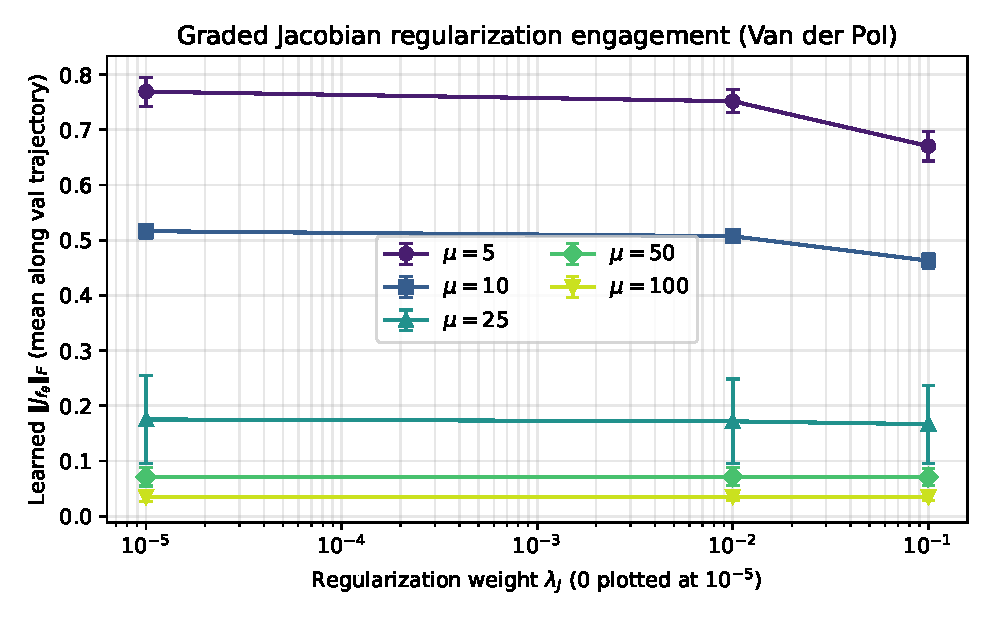
\includegraphics[width=0.7\textwidth]{figures/fig_engagement.pdf}
\caption{Engagement regime. Learned Jacobian Frobenius norm versus
  regularization weight $\lambda_J$, on Van der Pol at $\mu = 10$ (better-fit)
  and $\mu = 50$ (poorer-fit). Each point is the mean over 5 seeds; bars are
  $\pm 1$ std. At $\mu = 10$ the penalty suppresses $\|\fjac\|_F$ monotonically
  as $\lambda_J$ increases; at $\mu = 50$ the
  curve is essentially flat.}
\label{fig:engagement}
\end{figure}

\begin{table}[t]
\centering
\caption{Engagement regime data. Mean $\pm$ std over 5 seeds. Drop is
  computed against the $\lambda_J = 0$ baseline at the same $\mu$.}
\label{tab:engagement}
\begin{tabular}{c c r r r r}
\toprule
$\mu$ & $\lambda_J$ & $\|\fjac\|_F$ & Drop & $\NFE$ & $\mathrm{MSE}_\text{val}$ \\
\midrule
\multirow{3}{*}{10} & 0       & $0.5164 \pm 0.013$ & --        & $129.2 \pm 5.0$  & $1.184 \pm 0.020$ \\
                    & $10^{-2}$ & $0.5072 \pm 0.012$ & $1.78\%$  & $137.6 \pm 9.1$  & $1.229 \pm 0.067$ \\
                    & $10^{-1}$ & $0.4630 \pm 0.013$ & $\mathbf{10.35\%}$ & $132.8 \pm 9.9$  & $1.205 \pm 0.033$ \\
\midrule
\multirow{4}{*}{50} & 0          & $0.0714 \pm 0.017$ & --        & $141.2 \pm 27.6$ & $1.938 \pm 0.259$ \\
                    & $10^{-3}$  & $0.0713 \pm 0.016$ & $0.07\%$  & $140.0 \pm 26.2$ & $1.930 \pm 0.269$ \\
                    & $10^{-2}$  & $0.0715 \pm 0.016$ & $-0.20\%$ & $138.8 \pm 27.3$ & $1.928 \pm 0.269$ \\
                    & $10^{-1}$  & $0.0706 \pm 0.015$ & $\mathbf{1.04\%}$ & $136.4 \pm 26.0$ & $1.929 \pm 0.269$ \\
\bottomrule
\end{tabular}
\end{table}

\paragraph{Fit calibration against trivial predictors.}
The raw MSE values in Table~\ref{tab:engagement} are easier to interpret
relative to trivial validation-set predictors. On the same validation
trajectories, a zero-trajectory predictor obtains MSE $2.51 \pm 0.01$ at
$\mu = 10$ and $2.70 \pm 0.22$ at $\mu = 50$; an oracle constant predictor
using the validation-set mean obtains $2.51 \pm 0.01$ and $2.65 \pm 0.22$,
respectively. The learned \texttt{dopri5} baseline improves over this
constant predictor by $52.8\%$ at $\mu = 10$ but only $26.8\%$ at
$\mu = 50$. Thus ``poorer fit'' here means not only a larger absolute MSE,
but a substantially smaller reduction over a trivial constant trajectory.

\paragraph{Mechanism.}
The most plausible mechanism is that when the model fits the stiffer target
poorly, $f_\theta$ collapses toward a near-constant vector field whose
Jacobian norm is already much smaller than the network would need to
reproduce the true Van der Pol dynamics. At $\mu = 50$, $\|\fjac\|_F = 0.071$
is approximately one seventieth of the true Jacobian magnitude at the limit
cycle, which is of order $\mu$. The penalty term then has nothing to suppress.

\emph{Back-of-envelope.} At $\mu = 50$, $\lambda_J = 10^{-1}$, and
$\|\fjac\|_F = 0.071$, the penalty value is $\lambda_J \|\fjac\|_F^2 \approx
5.0 \times 10^{-4}$, while the task loss is $\approx 1.93$. The penalty
contributes a relative magnitude of order $2.6 \times 10^{-4}$ to the total
loss --- Adam's per-parameter gradient normalisation cannot amplify a signal
this small against the task gradient on every step. At $\mu = 10$ the same
calculation gives $0.1 \times 0.516^2 / 1.18 \approx 2.3 \times 10^{-2}$, two
orders of magnitude larger and within the regime where the penalty can
register at all. This calculation supports the engagement-gap mechanism.
Bumping the Hutchinson sample
count from $K = 1$ to $K = 4$ does not change this --- the variance of the
estimator is not the binding constraint --- and we report the $K = 4$ result
in Table~\ref{tab:k4}. The $\sim 1\%$ residual change is at the variance
floor of the experiment.

\paragraph{An alternative mechanism we cannot fully rule out.}
The penalty in our implementation is evaluated at sampled \emph{ground-truth}
trajectory points (\S\ref{sec:reg}), not along the model's predicted
trajectory. When the model is poorly fit (val\,MSE $= 1.94$ at $\mu = 50$),
its forward integration visits states quite different from the ground-truth
trajectory, so the penalty's gradient signal partially cancels with the
task-loss gradient pushing $f_\theta$ \emph{toward} the high-Jacobian true
dynamics. The augmented-state penalty integration of \citet{finlay2020train}
evaluates the penalty along the learned trajectory and would not suffer
this misalignment; we discuss this in \S\ref{sec:limitations}.

\begin{table}[t]
\centering
\caption{$K$ sweep at fixed $\lambda_J = 10^{-1}$, vdp $\mu = 50$, dopri5.
  Mean $\pm$ std over 5 seeds.}
\label{tab:k4}
\begin{tabular}{c r r}
\toprule
$K$ & $\|\fjac\|_F$ & Drop vs $\lambda_J = 0$ \\
\midrule
1 & $0.0706 \pm 0.015$ & $1.05\%$ \\
4 & $0.0704 \pm 0.016$ & $1.26\%$ \\
\bottomrule
\end{tabular}
\end{table}

\paragraph{Stiffness side-effect.}
At $\mu = 10$ where the penalty engages, $\NFE$ does \emph{not} decrease
(Table~\ref{tab:engagement}); if anything, $\NFE$ rises slightly. The learned
spectral stiffness ratio at $\mu = 10$ is $\approx 1.4$, indicating the
system is non-stiff at this $\mu$ value. The stability mechanism that
Proposition~\ref{prop:interaction} relies on (Appendix~\ref{app:interaction})
therefore does not apply: there is no stiff step-size restriction for the
penalty to relax. NFE is accuracy-limited in this regime, and the modest
penalty-induced changes in higher derivatives are within seed variance.

\subsection{H3: implicit-vs-explicit with a stiffness slope}
\label{sec:h3}

The proposal's ancillary hypothesis H3 asked whether an unregularized
explicit adaptive solver can match or beat a fixed-point implicit method at
matched validation MSE on a stiff Neural ODE. Extending the comparison across
$\mu \in \{25, 50, 100\}$ yields a clear slope (Table~\ref{tab:h3} and
Figure~\ref{fig:h3}). The wall-clock ratio
$W(\texttt{implicit\_adams})/W(\texttt{dopri5})$ grows monotonically from
$6.88\times$ at $\mu = 25$ to $7.89\times$ at $\mu = 100$ when ratios are
paired by seed. All three pairwise comparisons hit the $n = 5$ Wilcoxon floor
of $p = 0.031$ (one-sided, implicit slower) before correction; rank-biserial
effect size is $+1.0$ at each $\mu$ (all seeds in the same direction). Treated
as a three-comparison family, these $p$-values do not survive Bonferroni
correction.

\begin{table}[t]
\centering
\caption{H3 comparison across $\mu$: \texttt{dopri5} vs \texttt{implicit\_adams}
  at matched validation MSE on Van der Pol, $\lambda_J = 0$, 5 seeds each.
  The high-$\mu$ case is matched-bad rather than matched-good MSE.
  $\Delta\mathrm{MSE}$ is the percent difference in mean validation MSE
  between the two solvers (the matched-MSE precondition requires this to be
  small). Ratio is the mean of per-seed wall-clock ratios.}
\label{tab:h3}
\begin{tabular}{c r r r r r}
\toprule
$\mu$ & $W_\text{dopri5}$ (s) & $W_\text{implicit}$ (s) & Ratio & $\Delta\mathrm{MSE}$ & Wilcoxon $p$ \\
\midrule
25  & $0.0425 \pm 0.004$ & $0.2886 \pm 0.020$ & $6.88\times$ & $+2.44\%$ & $0.031$ \\
50  & $0.0430 \pm 0.006$ & $0.3083 \pm 0.009$ & $7.29\times$ & $+0.003\%$ & $0.031$ \\
100 & $0.0366 \pm 0.004$ & $0.2856 \pm 0.018$ & $7.89\times$ & $-0.003\%$ & $0.031$ \\
\bottomrule
\end{tabular}
\end{table}

\begin{figure}[t]
\centering
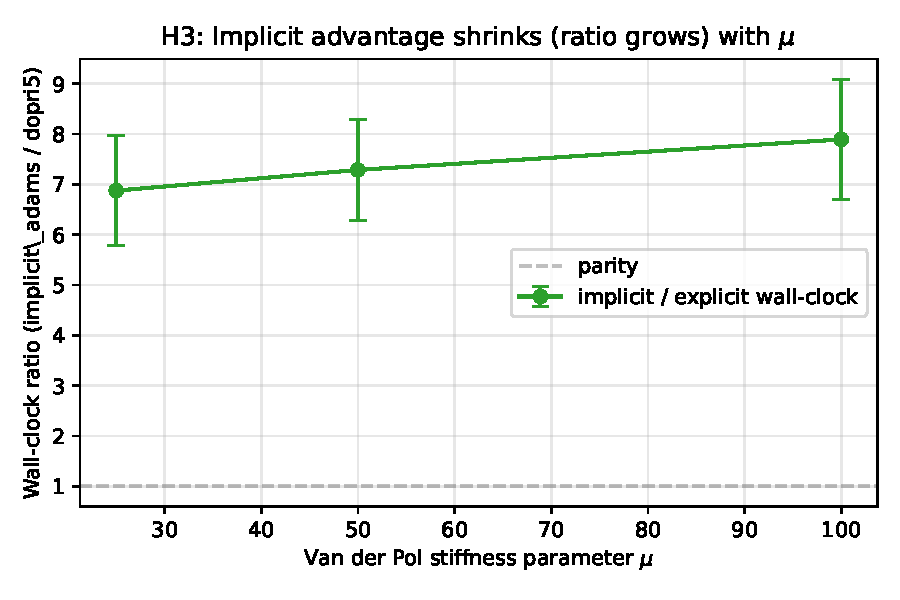
\includegraphics[width=0.65\textwidth]{figures/fig_h3_slope.pdf}
\caption{H3 stiffness slope. Wall-clock ratio of \texttt{implicit\_adams} to
  \texttt{dopri5} on Van der Pol as $\mu$ varies. The ratio grows monotonically,
  meaning the explicit adaptive solver's relative advantage \emph{increases}
  with target $\mu$ in this task family. Error bars are $\pm 1$ std over the
  5 seed-matched ratios.}
\label{fig:h3}
\end{figure}

\paragraph{Caveats on the slope.}
The naive prediction is the opposite of what we observe: as the system becomes
stiffer, the explicit adaptive solver should be forced into smaller steps for
stability, while the $A$-stable implicit method remains free to take large
steps. Three caveats apply to our inverted finding.

\emph{(i) The model fails to learn the stiff dynamics.}
As $\mu$ rises, $f_\theta$ becomes a low-norm approximation that is easy to
integrate for any solver. Validation MSE grows from $1.65$ at $\mu = 25$ to
$2.38$ at $\mu = 100$. The learned spectral stiffness ratio at $\mu = 100$
can be enormous numerically (driven by near-singular eigenvalues), but this
is an artefact of poor fit rather than learned stiff dynamics. The
matched-MSE precondition holds across our $\mu$ values (Table~\ref{tab:h3}),
but at $\mu = 100$ it is matched at $\mathrm{MSE} \approx 2.38$ ---
\emph{matched-bad} accuracy, not matched-good accuracy. The slope statement
should therefore be read as: ``on a poorly-fit network whose effective
stiffness grows weakly with target $\mu$, the wall-clock ratio of these two
solvers grows monotonically.''

\emph{(ii) The integration horizon co-varies with $\mu$.}
Our time grid sets $T_\text{end} = \max(20, 2\mu)$ (\S\ref{sec:tasks}), so the
integration span grows linearly with $\mu$: $T_\text{end} = 50$ at $\mu = 25$,
$100$ at $\mu = 50$, $200$ at $\mu = 100$. Fixed-step contributions to NFE
scale linearly with $T_\text{end}$, while adaptive contributions scale
sub-linearly. Part of the apparent slope --- though not all of it, since
\texttt{dopri5} NFE is itself roughly flat across $\mu$
(Table~\ref{tab:h3} columns show wall-clock per forward pass, not NFE per
unit integration time) --- is therefore attributable to the horizon
confound rather than to stiffness.

\emph{(iii) The implicit baseline is fixed-point, not Newton-based.}
\texttt{torchdiffeq.implicit\_adams} pays the per-step cost of an implicit
method (many $f$ evaluations per fixed-point sweep) without exploiting the
$A$-stability benefit a Newton-based BDF or Radau IIA would deliver. Our
H3 result therefore says: for practitioners in the \texttt{torchdiffeq}
ecosystem on mildly stiff Neural ODEs, switching to \texttt{implicit\_adams}
is a wall-clock regression, not an improvement. It does not say that
implicit integration in general is a bad idea on stiff Neural ODEs.

\subsection{H1 and H2: null results with mechanism}
\label{sec:null}

The proposal's preregistered hypotheses H1 (NFE reduction larger on stiff
than smooth targets) and H2 (stiffness suppression larger on stiff targets)
are \emph{not} supported by our data. At the originally-preregistered
$\mu = 50$, $\lambda_J = 10^{-3}$ setting, the regularization is operationally
inert (Table~\ref{tab:engagement}). Extending the sweep to $\lambda_J = 10^{-1}$
and $K = 4$ does not rescue H1: the residual $\Delta\NFE$ between $\lambda_J =
0$ and $\lambda_J = 10^{-1}$ at $\mu = 50$ is $\approx 5$ NFE on a baseline
of $141 \pm 28$ NFE --- well within seed noise. Running the sweep at
$\mu = 10$ where the penalty does engage produces no NFE reduction either,
because the system is non-stiff at that $\mu$ value.

We interpret the null as a \emph{failure of observed regime overlap}: in this
setup, the penalty engages where the learned dynamics are not stiff enough to
produce an NFE benefit, and is inert in the stiffer setting where such a
benefit would be most useful.
Proposition~\ref{prop:interaction} (Appendix~\ref{app:interaction}) predicts
a positive interaction only \emph{conditional} on engagement, an assumption
that fails on this task family; the proposition therefore does not constrain
our null result, but neither is it falsified --- it survives only as a
hypothesis for a hypothetical regime where penalty and stiffness co-engage.

\paragraph{Preregistration deviation.}
The proposal preregistered $\lambda_J$ selection on validation MSE within
$5\%$ of the baseline, then comparing NFE at that selected $\lambda_J$.
Because no tested $\lambda_J$ at $\mu = 50$ produced a meaningful change in
either the validation MSE or the Jacobian Frobenius norm, we report the full
sweep (Table~\ref{tab:engagement}) rather than a single selected $\lambda_J$.
A faithful reading of the preregistered protocol would select $\lambda_J = 0$
(lowest val MSE at every $\mu$), in which case there is no ``regularized''
cell to compare against the baseline. We view the full sweep as the
informationally richer report.

\section{Discussion}
\label{sec:discussion}

\paragraph{The penalty--fit--stiffness trade-off.}
Our findings, taken together, suggest a structural trade-off that governs
when Jacobian regularization is useful for Neural ODEs:
\begin{enumerate}[leftmargin=2em]
\item The penalty has a soft-Lipschitz interpretation
  (Lemma~\ref{lem:frob-dominates}, Appendix~\ref{app:frobenius-bound}): it
  upper-bounds the spectral radius of $\fjac$. This control is indirect and
  potentially loose: reducing $\|\fjac\|_F$ reduces an upper bound on
  $\rho(\fjac)$, but it does not specifically target the fast/slow eigenvalue
  structure that makes a system stiff, nor does it guarantee lower solver
  cost. The penalty therefore has an \emph{engagement requirement}: the
  network must have learned a high-norm vector field for the penalty to have
  something to suppress.
\item Engagement requires \emph{fit}: the network must have fit the target
  well enough that $f_\theta$ has built up the Lipschitz constant of the
  target, otherwise it collapses to a low-norm field that the penalty cannot
  meaningfully shape.
\item In these runs, higher target stiffness is precisely where fit degrades
  under standard training~\citep{kim2021stiff}: the learned vector field falls
  into a low-fit, low-Jacobian-norm regime, exactly where the penalty becomes
  inert. (Note that the underlying mechanism for the training difficulty
  differs from~\citet{kim2021stiff}, who identify adjoint-system stiffness;
  the \emph{low-Lipschitz collapse} we observe is a complementary failure mode
  that prevents the penalty from engaging whether or not the adjoint is
  stable.)
\end{enumerate}
The three-way trade-off suggests that Jacobian regularization in this setup
helps most where it is least needed (well-fit, non-stiff systems) and helps
least where it is most needed (poorly-fit, stiff systems). This is consistent
with the positive results in \citet{finlay2020train}, where the
density-estimation tasks afford good fit, and with the training-difficulty
results in \citet{kim2021stiff}.

\paragraph{Implications for the implicit alternative.}
Our H3 result that explicit adaptive integration beats fixed-point implicit
integration at every tested $\mu$ does not generalise to all implicit
methods; in particular, a Newton-based BDF or Radau~IIA implementation may
recover the $A$-stability advantage. The takeaway from H3 in its current
scope is more limited but still useful: for practitioners using
torchdiffeq's ecosystem, switching to \texttt{implicit\_adams} on mildly
stiff Neural ODEs is a wall-clock regression, not an improvement.

\section{Limitations and Future Work}
\label{sec:limitations}

\paragraph{Single architecture.}
All experiments use a 2-hidden-layer MLP of width 64 with $\tanh$
activations. A wider or deeper network might develop sufficient Lipschitz
constant on Van der Pol at $\mu = 50$ to fall back into the engagement
regime; this is an important sweep for future work.

\paragraph{Single optimiser.}
Adam adapts the per-parameter learning rate using gradient statistics, which
could amplify or attenuate the penalty gradient relative to the task gradient
in ways that are not transparent. Comparing against SGD with momentum (and
optionally a learning-rate decay schedule) would isolate the optimiser's role
from the penalty's role.

\paragraph{Single stiff system.}
Van der Pol is a 2D limit-cycle system with parameterised stiffness; the
engagement regime we identified may be specific to this geometry. Robertson
kinetics~\citep{robertson1966solution} provides a much stiffer
$d = 3$ alternative and would test whether the trade-off holds beyond limit
cycles.

\paragraph{Single implicit method.}
\texttt{implicit\_adams} is fixed-point, not Newton-based. A proper
comparison to $A$-stable Newton-based implicit methods (e.g., Kvaerno5 in
\texttt{diffrax}, BDF in \texttt{torchode}, or Radau in
\texttt{DifferentialEquations.jl}~\citep{rackauckas2017differentialequations})
is needed before strong claims about implicit-vs-explicit can be made on
stiff Neural ODEs.

\paragraph{Five seeds.}
$n = 5$ pairs are sufficient for one-tailed Wilcoxon to reach the floor
$p = 0.031$ when all seeds agree, but insufficient to resolve interactions
that are smaller than the standard deviation. Where we observed flat or
inconsistent effects (e.g., the $1\%$ residual at $\mu = 50$), an $n = 20$
seed budget would more decisively rule out a small effect.

\paragraph{Adaptive step-size logging.}
For adaptive solvers we report only the mean step size (derived from NFE);
the min, max, and variance require monkey-patching torchdiffeq's internal
step-acceptance loop. The full distribution would enable the step-size
histogram plot proposed in the original design but is not load-bearing for
the central claims.

\paragraph{Integration-horizon confound in the $\mu$ sweep.}
Our default time grid scales as $T_\text{end} = \max(20, 2\mu)$, so the
$\mu$ sweep co-varies integration span with stiffness (Section~\ref{sec:h3}).
A cleaner H3 sweep would fix $T_\text{end}$ across $\mu$ values --- e.g.,
$T_\text{end} = 50$ everywhere --- to isolate the stiffness effect from the
horizon effect.

\paragraph{Raw time-input confound.}
The vector field receives raw time $t$ as an input feature. Because
$T_\text{end}$ scales with $\mu$, the range of the time feature also grows with
target stiffness, potentially changing the optimisation problem independently
of stiffness itself. A cleaner follow-up would either normalise time to
$[0,1]$ for every $\mu$ value or compare against an autonomous vector field
that does not receive $t$.

\paragraph{Ground-truth penalty sampling and the augmented-state alternative.}
We sample penalty evaluation points from the ground-truth training trajectory
rather than along the predicted learned trajectory (\S\ref{sec:reg}). On a
well-fit network the two distributions are close, but on a poorly-fit
network they diverge --- the model's forward integration visits states that
the penalty is not evaluated at, decoupling the penalty's gradient signal
from the trajectory whose cost the user cares about. The augmented-state
penalty integration of~\citet{finlay2020train} avoids this by computing
$\int_0^T \|\fjac(x_t, t)\|_F^2 dt$ along the learned trajectory inside the
ODE solve; we did not implement this variant, and our engagement-gap
mechanism therefore conflates two contributing causes: (a) low-Lipschitz
collapse of $f_\theta$, and (b) misalignment between penalty support and
learned trajectory. A clean separation of these mechanisms is the most
important methodology improvement for future work.

\paragraph{Levers that could relax the trade-off.}
Future work could attempt to relax any of the three legs of the
penalty--fit--stiffness trade-off (\S\ref{sec:discussion}):
\begin{itemize}[leftmargin=2em]
\item Replace the soft Frobenius penalty by hard Lipschitz constraints
  (spectral normalisation per layer, or projected gradient onto a
  Lipschitz-bounded set), which would shape $f_\theta$ even when the
  unconstrained optimum is low-Lipschitz.
\item Use the augmented-state penalty integration of \citet{finlay2020train}
  so the penalty is evaluated along the learned trajectory.
\item Loss-normalised regularization: replace $\lambda_J$ by
  $\lambda_J \cdot \texttt{detach}(\mathcal{L}_\text{task})^{-1}$ so the
  penalty is scale-invariant to a difficult task loss.
\item Specialised training for stiff Neural ODEs as in \citet{kim2021stiff}
  (adjoint stabilisation, time-rescaling) to push the fit-vs-stiffness
  boundary outward.
\end{itemize}

\section{Conclusion}
\label{sec:conclusion}

The preregistered question was whether Jacobian regularization reduces
Neural ODE solver cost more on stiff systems than on smooth ones. The
preregistered factorial returned a null. The four follow-up sweeps reframe
the null as a \emph{penalty--fit--stiffness trade-off}: regularization
requires fit, while higher target stiffness coincides with poorer fit in this
training setup, and on this task family the two regimes do not overlap. Future
work that breaks the trade-off via
hard Lipschitz constraints, augmented-state penalty integration, or
specialised training for stiff Neural ODEs is the natural next step. All
115 result JSONs, configuration files, and theoretical derivations are
bundled with this paper.

\bibliographystyle{plainnat}
\bibliography{refs}

% Appendix - Theoretical Derivations
% Marked separately so it can be transcribed by hand at the end of the project.

\appendix

\section{Theoretical Derivations}
\label{app:theory}

This appendix collects the analytical results that motivate the experimental design.
Where a result is classical, we cite the canonical source and give a compact
derivation suitable for transcription by hand. Where the result is a novel synthesis
of standard pieces, we mark it with a $\star$.

Throughout this appendix, $f \colon \mathbb{R}^d \to \mathbb{R}^d$ is the (autonomous)
vector field of the ODE $\dot x = f(x)$, and $J(x) = \partial f / \partial x$ is its
Jacobian.

\subsection{Linear stability and the step-size restriction (Mechanism B)}
\label{app:stability}

\begin{theorem}[Stability step bound, after Hairer--Wanner~\cite{hairer1996solving}]
\label{thm:stability}
Let $\Phi_h$ be an explicit Runge--Kutta method with stability region $S \subset
\mathbb{C}$, and apply it to the linear test equation $\dot y = \lambda y$.
The numerical scheme is stable iff $h\lambda \in S$. For a nonlinear system
$\dot x = f(x)$ in the neighbourhood of a point $x^\star$ where $f(x^\star) = 0$,
local stability of $\Phi_h$ requires
\begin{equation}
h \cdot \rho(J(x^\star)) \;\leq\; C_p,
\label{eq:stability-bound}
\end{equation}
where $\rho(\cdot)$ denotes spectral radius and $C_p$ is a method-dependent constant
(for classical RK4, $C_p \approx 2.78$ on the negative real axis).
\end{theorem}

\begin{proof}[Sketch]
The standard linearisation argument: write $x = x^\star + y$, expand
$f(x^\star + y) = J(x^\star) y + O(\|y\|^2)$, and apply $\Phi_h$ to the linearised
system. Stability is then a property of the eigenvalues of the amplification matrix
$R(hJ)$, which equals $\Phi_h$ applied to $\dot y = \lambda y$ for each eigenvalue
$\lambda$ of $J(x^\star)$. The condition $h\lambda \in S$ is therefore necessary and
sufficient for local linear stability. See~\cite{hairer1996solving} \S IV.2 for the
full argument.
\end{proof}

\textbf{Consequence.} On a \emph{stiff} system, $\rho(J) \gg 1$, so the stable step
size $h_\text{stab} = C_p / \rho(J)$ can be much smaller than the step size required
for accuracy alone. This is the mechanism that explicit methods are penalised on
stiff problems.

\subsection{Frobenius norm bounds the spectral radius}
\label{app:frobenius-bound}

\begin{lemma}[Frobenius dominance]
\label{lem:frob-dominates}
For any matrix $A \in \mathbb{R}^{d \times d}$,
\begin{equation}
\rho(A) \;\leq\; \|A\|_2 \;\leq\; \|A\|_F,
\label{eq:frob-bound}
\end{equation}
with equality in the first inequality iff $A$ is normal, and equality in the second
iff $A$ has at most one nonzero singular value.
\end{lemma}

\begin{proof}
Let $\sigma_1 \geq \dots \geq \sigma_d \geq 0$ be the singular values of $A$. Then
$\|A\|_2 = \sigma_1$ and $\|A\|_F^2 = \sum_i \sigma_i^2$, so
$\|A\|_2 \leq \|A\|_F$. For any eigenvalue $\lambda$ of $A$ with eigenvector $v$,
$\|Av\| = |\lambda| \|v\|$, hence $|\lambda| \leq \|A\|_2$. Taking the maximum over
eigenvalues yields $\rho(A) \leq \|A\|_2$.
\end{proof}

\textbf{Consequence.} The penalty $\lambda_J \|J\|_F^2$ is a soft, differentiable
upper bound on $\lambda_J \rho(J)^2$. Suppressing $\|J\|_F$ therefore relaxes the
stability restriction~\eqref{eq:stability-bound}.

\subsection{Truncation-error step bound (Mechanism A)}
\label{app:trunc-bound}

\begin{theorem}[Accuracy step bound, after Hairer--N\o{}rsett--Wanner~\cite{hairer1993solving}]
\label{thm:accuracy}
For an order-$p$ Runge--Kutta method with adaptive step size satisfying a
relative-error tolerance $\tau$, the expected number of steps to integrate over
$[0, T]$ obeys
\begin{equation}
N \;\leq\; C \cdot T \cdot M^{p/(p+1)} \cdot \tau^{-1/(p+1)},
\label{eq:accuracy-bound}
\end{equation}
where $M = \sup_{t \in [0,T]} \|x^{(p+1)}(t)\|$ and $C$ depends only on the method.
\end{theorem}

\begin{proof}[Sketch]
The local truncation error of an order-$p$ method is
$\tau_n = \frac{h^{p+1}}{(p+1)!} x^{(p+1)}(\xi_n) + O(h^{p+2})$ for some
$\xi_n \in [t_n, t_{n+1}]$. The optimal adaptive step satisfies
$h^{p+1} M \approx \tau$, so $h \approx (\tau / M)^{1/(p+1)}$. The number of steps is
$N \approx T / h$. See~\cite{hairer1993solving} \S II.4.
\end{proof}

\textbf{Consequence.} Since $x^{(p+1)}$ is a polynomial in $J$ and its derivatives,
suppressing $\|J\|$ reduces $M$ and therefore $N$. This is the accuracy-side
benefit of Jacobian regularization, in contrast to the stability-side benefit of
\S\ref{app:stability}.

\subsection{Hutchinson estimator for the Frobenius norm squared}
\label{app:hutchinson}

\begin{theorem}[Hutchinson unbiasedness, after Hutchinson~\cite{hutchinson1990stochastic}]
\label{thm:hutchinson}
Let $A \in \mathbb{R}^{d \times d}$ and let $\epsilon \in \mathbb{R}^d$ be a random
vector with $\mathbb{E}[\epsilon] = 0$ and $\mathbb{E}[\epsilon \epsilon^\top] = I_d$
(e.g., $\epsilon$ has i.i.d.\ Rademacher entries, or i.i.d.\ $\mathcal{N}(0,1)$).
Then
\begin{equation}
\mathbb{E}_\epsilon\!\left[\|A^\top \epsilon\|^2\right] \;=\; \|A\|_F^2.
\label{eq:hutchinson}
\end{equation}
\end{theorem}

\begin{proof}
\begin{align}
\mathbb{E}_\epsilon\!\left[\|A^\top \epsilon\|^2\right]
&= \mathbb{E}\left[\epsilon^\top A A^\top \epsilon\right]
 = \mathbb{E}\!\left[\mathrm{tr}\!\left(A A^\top \epsilon \epsilon^\top\right)\right] \\
&= \mathrm{tr}\!\left(A A^\top \, \mathbb{E}[\epsilon \epsilon^\top]\right)
 = \mathrm{tr}(A A^\top)
 = \|A\|_F^2.
\end{align}
\end{proof}

\textbf{Variance bound.} For Rademacher $\epsilon$,
$\mathrm{Var}[\|A^\top \epsilon\|^2] = 2 \sum_{i \neq j} (AA^\top)_{ij}^2$, which is
zero iff $AA^\top$ is diagonal. A $K$-sample average reduces variance by $1/K$.

\textbf{Implementation.} In automatic differentiation, $A^\top \epsilon$ is the
vector--Jacobian product of $f$ at the evaluation point with co-tangent vector
$\epsilon$, which costs a single backward pass through $f$ regardless of $d$.

\subsection{A-stability of implicit Euler}
\label{app:a-stability}

\begin{theorem}[A-stability of implicit Euler, after Dahlquist~\cite{dahlquist1963special}]
\label{thm:a-stability}
The implicit Euler method $x_{n+1} = x_n + h f(x_{n+1})$ applied to the linear test
equation $\dot y = \lambda y$ with $\mathrm{Re}(\lambda) < 0$ is stable for every
$h > 0$.
\end{theorem}

\begin{proof}
On $\dot y = \lambda y$, the scheme reduces to $y_{n+1} = y_n + h \lambda y_{n+1}$,
so $y_{n+1} = (1 - h\lambda)^{-1} y_n$. For $\mathrm{Re}(\lambda) < 0$,
$|1 - h\lambda|^2 = (1 - h\mathrm{Re}(\lambda))^2 + (h\mathrm{Im}(\lambda))^2 > 1$
for all $h > 0$, hence $|1 - h\lambda|^{-1} < 1$ and $|y_{n+1}| < |y_n|$. The scheme
is therefore stable for all $h > 0$. Moreover $|1 - h\lambda|^{-1} \to 0$ as
$h \to \infty$, so the method is also L-stable.
\end{proof}

\textbf{Consequence.} On a stiff system, the implicit Euler step size is governed
only by accuracy (Mechanism A), not by stability (Mechanism B). Each step, however,
requires solving a nonlinear equation; for a Newton-based implicit solver this is
$O(\bar K)$ Jacobian evaluations and linear solves per step.

\subsection{The interaction prediction $\star$}
\label{app:interaction}

We now combine the preceding results to derive the prediction that motivated the
original H1 hypothesis. Define the NFE reduction at matched validation MSE as
$\Delta N(s) := N_\text{base}(s) - N_\text{reg}(s)$ where $s$ indexes target-system
stiffness. Suppose (i) the regularizer reduces $\|J_{f_\theta}\|_F$ by a
multiplicative factor $\beta \in (0,1)$ relative to baseline, (ii) the smooth task is
accuracy-limited, and (iii) the stiff task is stability-limited.

By Theorem~\ref{thm:accuracy}, on the smooth task
\begin{equation*}
\frac{N_\text{reg}}{N_\text{base}}
  = \left(\frac{M_\text{reg}}{M_\text{base}}\right)^{p/(p+1)}
  \approx \beta^{p/(p+1)},
\end{equation*}
so $\Delta N_\text{smooth} \propto (1 - \beta^{p/(p+1)})$.

By Theorem~\ref{thm:stability}, on the stiff task
$N \propto T \cdot \rho(J) / C_p$ and Lemma~\ref{lem:frob-dominates} gives
$\rho(J) \leq \|J\|_F$, so
\begin{equation*}
\frac{N_\text{reg}}{N_\text{base}} \approx \beta,
\end{equation*}
yielding $\Delta N_\text{stiff} \propto (1 - \beta)$.

\begin{proposition}[Predicted interaction]
\label{prop:interaction}
Under assumptions (i)--(iii),
\begin{equation}
\frac{\Delta N_\text{stiff}}{\Delta N_\text{smooth}}
  \;\approx\; \frac{1 - \beta}{1 - \beta^{p/(p+1)}}
  \;>\; 1 \quad \text{for } p \geq 1.
\label{eq:interaction-prediction}
\end{equation}
\end{proposition}

\textbf{Empirical caveat.} Assumption (i) requires the regularizer to engage at the
training operating point; \S\ref{sec:engagement} of the main text shows this
assumption \emph{fails} on the stiff target used here, because the model never
develops the high-Lipschitz vector field that the penalty would suppress.
\textbf{Proposition~\ref{prop:interaction} is therefore predictively vacuous
on this task family:} its antecedent has empirical probability zero on
Van der Pol $\mu \geq 25$, so the proposition does not constrain our null
result, but neither is it falsified. It survives as a hypothesis for a
hypothetical regime where penalty and stiffness co-engage.

\subsection{Cost decomposition for implicit Runge--Kutta}
\label{app:implicit-cost}

\begin{proposition}[Implicit cost decomposition]
\label{prop:implicit-cost}
For an $s$-stage implicit Runge--Kutta method run for $N$ outer steps, with average
Newton iteration count $\bar K$ per step, the cumulative work is
\begin{equation}
W \;=\; N \cdot \bar K \cdot \bigl[s \cdot W_f \;+\; W_J \;+\; W_\text{lin}\bigr],
\label{eq:implicit-cost}
\end{equation}
where $W_f$ is the cost of one $f$ evaluation, $W_J$ the cost of one Jacobian
evaluation, and $W_\text{lin}$ the cost of a single linear solve of dimension
$d \cdot s$.
\end{proposition}

Equation~\eqref{eq:implicit-cost} is the unit in which implicit and explicit costs
should be compared. In particular, the NFE count alone (which is $N \cdot \bar K
\cdot s$ for implicit methods) is not sufficient to characterise the wall-clock
cost; the Jacobian and linear-solve terms can dominate on small $d$ where dense
linear algebra is cheap but $W_J$ is non-trivial.

\section{Reproducibility Checklist}
\label{app:reproducibility}

This checklist records settings not already stated in \S\ref{sec:methods}; we
do not duplicate model, optimiser, training, or solver descriptions that
appear in the main text.

\begin{enumerate}[leftmargin=2em]
\item \textbf{Software.} Python 3.10.5, PyTorch 2.11.0, torchdiffeq
0.2.5~\citep{chen2018torchdiffeq}, NumPy 2.2.6, SciPy 1.15.3,
matplotlib 3.10.9. Hardware: Apple Silicon laptop, CPU-only training.
Total wall time for the 115-cell sweep: $\approx 8$ hours.
\item \textbf{Wall-clock measurement protocol.} Each cell's reported
wall-clock per forward pass is a single timed call to
\texttt{model(x0\_val, t)} under \texttt{torch.no\_grad()}, with no warm-up
pass. On CPU this is noisy at the millisecond level; we recommend
reproducing with at least three timed passes per cell if precise wall-clock
numbers matter to the downstream conclusion.
\item \textbf{IC generator ordering.} For each seed, a single
\texttt{torch.Generator(seed)} is used to draw the $256$ training $x_0$
samples and then the $64$ validation samples (disjoint, consecutive draws
from the same generator). The global PyTorch RNG is independently seeded
with the same integer for model initialisation and Hutchinson noise.
\item \textbf{Penalty sampling distribution.} 32 $(t, x)$ pairs per training
step are drawn uniformly from the \emph{flat} $(T \cdot B)$ index of
ground-truth training trajectories, so time and initial-condition indices
are sampled jointly with equal weight. This implicitly over-samples
slow-manifold portions of the Van der Pol trajectory where the
uniform-in-$t$ grid is dense.
\item \textbf{Tolerance sweep coupling.} $r_\text{tol}$ and $a_\text{tol}$
are both varied in the tolerance sweep:
$(r_\text{tol}, a_\text{tol}) \in \{(10^{-3}, 10^{-5}), (10^{-5}, 10^{-7}),
(10^{-7}, 10^{-9})\}$. The fitted exponent $\alpha$ in \S\ref{sec:h0}
therefore reflects sensitivity to both tolerances jointly. The tolerance
override is applied before training, so these cells are train-and-evaluate
tolerance settings rather than an eval-only sweep on one fixed trained model.
\item \textbf{Solver-registry mutation.} Tolerance overrides are implemented
by in-process mutation of \texttt{SOLVER\_REGISTRY} in
\texttt{scripts/train\_single.py}. Each cell runs in a fresh subprocess
(via \texttt{run\_matrix.py}) so the mutation does not leak across cells.
\item \textbf{Statistical tests.} Paired Wilcoxon signed-rank with the
\emph{wilcox} zero-handling convention; rank-biserial correlation as effect
size. Bonferroni correction is applied at family-wise $\alpha = 0.05$
across the H3 set ($m = 3$). With each H3 comparison hitting one-sided
$p = 0.031$ uncorrected, none survives Bonferroni at $\alpha/m = 0.017$
when treated as a family. We therefore report the consistent direction
across $\mu$ as the substantive finding, not the per-comparison
significance after correction.
\item \textbf{Result provenance.} Result filenames encode task, solver,
$\lambda_J$, and seed; full metadata such as $\mu$, $K$, tolerance overrides,
and the output directory for follow-up sweeps must be read from the JSON
\texttt{config} block and directory structure. A cleaner archival release
would include a manifest or filenames containing every experimental factor.
\item \textbf{Total cells.} 115 trained runs across all sweeps,
summarised in Table~\ref{tab:cells} of the main text.
\end{enumerate}


\end{document}
